\documentclass[letterpaper]{article}

\usepackage{graphicx}
\usepackage[letterpaper, left=30mm, right=30mm, top=30mm, bottom=30mm]{geometry}

\begin{document}

\begin{flushright}
	
\includegraphics[width=5cm, height=4cm]{Imagenes/logoMATCOM.png}\\
	{\scriptsize \textbf{Facultad de Matemática y Computación}}
\end{flushright}

\

\

\begin{center}
	\textbf{{\Huge PROYECTO DE }}
	
	\

	\textbf{{\Huge PROGRAMACIÓN II}}
	\

	\

	\

	\

	\

	\

	\

	\

	\

	\textbf{{\Huge H U L K}}

	\
	
	\textbf{{\LARGE Havana University Language for Kompilers}}
\end{center}

\begin{figure}[b]
	\begin{flushleft}
		{\huge \textbf{Estudiante:} \textit{Claudia Hernández Pérez}}

		\
	
		{\LARGE \textbf{Grupo:} \textit{C-113}}
	\end{flushleft}
\end{figure}

\newpage
{\small
HULK es un lenguaje de programación imperativo, funcional, estática y fuertemente tipado. Casi todas las instrucciones en HULK son expresiones. 
En particular, el subconjunto de HULK que usted implementar se compone solamente de expresiones que pueden escribirse en una línea. \\

\textbf{{\large $\circ $  Tipos Básicos}}\\

El lenguaje HULK contiene tres tipos básicos: 'string', 'boolean' y 'number'.

\begin{center}
	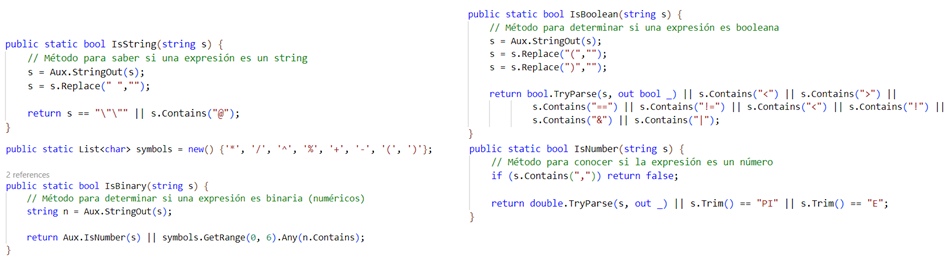
\includegraphics[width=13cm, height=4.25cm]{Imagenes/Types.png}\\
	{\scriptsize \textbf{Fig 1.1 Identificación de tipos básicos del lenguaje}}
\end{center}

La jerarquía de símbolos es: \\
• Símbolos de tipo 'number' : $\wedge$'; '*', '/' y '\%'; '+' y '-' \\
• Símbolos de tipo 'boolean':  '!'; '$>$', '$<$', '$>=$' y '$<=$'; '==' y '!='; '\&' y '$|$' \\
• Símbolos de tipo 'string' : '@' \\

De forma recursiva se procede en sentido contrario a la jerarquía, de forma que se va descomponiendo la expresión desde la operación más interna a la más externa.
La expresión se va evualuando en dos miembros, excepto el '!' que solo admite miembro derecho, hasta hacerla tan pequeña 
  
{\normalsize}

\begin{center}
\end{center}


\textbf{{\large $\circ $ }}\\



\begin{center}
\end{center}


\begin{center}
\end{center}



\textbf{{\large $\circ $ }}\\


\begin{center}
\end{center}



\

\textbf{{\large $\circ $ }}\\



\begin{center}
\end{center}


\begin{center}
\end{center}



\begin{center}
\end{center}


\begin{center}
\end{center}

\textbf{{\large $\circ $}}\\


\textbf{{\large $\circ $}}\\


}
\begin{center}
\end{center}

\end{document}